\documentclass[onecolumn, draftclsnofoot,10pt, compsoc]{IEEEtran}
\usepackage{graphicx}
\usepackage{url}
\usepackage{setspace}
\usepackage{longtable}

\usepackage{geometry}
\geometry{textheight=9.5in, textwidth=7in}

% 1. Fill in these details
\def \CapstoneTeamName{		}
\def \CapstoneTeamNumber{		6}
\def \GroupMemberOne{			Donghao Lin}
\def \GroupMemberTwo{			Joshua Diedrich}
\def \GroupMemberThree{			Christopher Breniser}
\def \CapstoneProjectName{		Race Car Scanning and Modeling}
\def \CapstoneSponsorCompany{	REHV}
\def \CapstoneSponsorPersonOne{	Kyson Montague}
\def \CapstoneSponsorPersonTwo{	Rodney Stauber}

% 2. Uncomment the appropriate line below so that the document type works
\def \DocType{	
				%Requirements Document
				%Technology Review
				%Design Document
				Progress Report
				}
			
\newcommand{\NameSigPair}[1]{\par
\makebox[2.75in][r]{#1} \hfil 	\makebox[3.25in]{\makebox[2.25in]{\hrulefill} \hfill		\makebox[.75in]{\hrulefill}}
\par\vspace{-12pt} \textit{\tiny\noindent
\makebox[2.75in]{} \hfil		\makebox[3.25in]{\makebox[2.25in][r]{Signature} \hfill	\makebox[.75in][r]{Date}}}}
% 3. If the document is not to be signed, uncomment the RENEWcommand below
%\renewcommand{\NameSigPair}[1]{#1}

%%%%%%%%%%%%%%%%%%%%%%%%%%%%%%%%%%%%%%%
\begin{document}
\begin{titlepage}
    \pagenumbering{gobble}
    \begin{singlespace}
    	
\includegraphics[height=4cm]{coe_v_spot1}
        \hfill 
        % 4. If you have a logo, use this includegraphics command to put it on the coversheet.
        %\includegraphics[height=4cm]{CompanyLogo}   
        \par\vspace{.2in}
        \centering
        \scshape{
            \huge CS Capstone \DocType \par
            {\large\today}\par
            \vspace{.5in}
            \textbf{\Huge\CapstoneProjectName}\par
            \vfill
            {\large Prepared for}\par
            \Huge \CapstoneSponsorCompany\par
            \vspace{5pt}
            {\Large\NameSigPair{\CapstoneSponsorPersonOne}\par}
            {\Large\NameSigPair{\CapstoneSponsorPersonTwo}\par}
            {\large Prepared by }\par
            Group\CapstoneTeamNumber\par
            % 5. comment out the line below this one if you do not wish to name your team
            \CapstoneTeamName\par 
            \vspace{5pt}
            {\Large
                \NameSigPair{\GroupMemberOne}\par
                \NameSigPair{\GroupMemberTwo}\par
                \NameSigPair{\GroupMemberThree}\par
            }
            \vspace{20pt}
        }
        \begin{abstract}
        % 6. Fill in your abstract 
        	This document describes the method used to measure the distance from a set point to an Indy Lights race car wheel using stereo vision distance scanning. This document will explore our progress to up to the end of winter term 2019. We will go over the OpenCV libraries and functions used, as well as the formulas created to calculate Indie Lights race cars axle length.
        \end{abstract}     
    \end{singlespace}
\end{titlepage}
\newpage
\pagenumbering{arabic}
\tableofcontents
% 7. uncomment this (if applicable). Consider adding a page break.
%\listoffigures
%\listoftables
\clearpage

\section{Purpose/Goals}
Our project is based around the idea of supplementing a process that Race Cars undergo before each race, referred to as a pre-race inspection.  Specifically, our project works on a car called an Indy Light.  An Indy Light is a certain type of race car, similar to that of an Indy Car.  Prior to each race, every Indy Light car must meet certain requirements to pass inspection.  These requirements include things like weight, width, tire pressure, wing angle, and many more.  An inspection starts with the vehicle being rolled onto a scale.  Next, the inspection team takes each required measurement of the car by hand, using special tooling.  The car then either passes or fails it’s inspection.
\newline

\noindent The purpose of our project is to supplement the pre-race inspection process using automated technology.  It takes a lot of manpower, and tedious work to make each measurement on the car.  Having people manually using tools to make every measurement makes for a somewhat slow inspection.  Our project aims at replacing some of these manual measurements with automated ones.  This should reduce the man-power needed to obtain measurements, and make it as easy as clicking a button.  Our device should also add to the process by measuring a few things that the team is not already picking up.
\newline

\noindent The first measurements we want to make are called camber and toe.  These relate to the wheels of the vehicle, specifically their angle.  Wheels are not all pointed straight forward and straight up and down, they often have some angle associated with them. Camber is the vertical angle of the wheel, while toe is the horizontal angle of the wheel.
\newline

\noindent Next we want to measure the wheelbase of the car.  The wheelbase is the distance from the center axle of the front wheels to the center axle of the back wheels.
\newline

\noindent Finally,  we want to measure what is called the track.  Track is basically the width of the car.  It is the distance horizontally from wheel to wheel.  This measurement is especially difficult to take by hand, because you can't just spread a measuring tape from one wheel across the car to the other.
\newline

\noindent The measurements we are taking are going to be very important.  Inspection for each car can actually stop that car from competing in the race, which is a big deal for the driver or company associated with that car.  Because of that, our system needs to meet strict goals when it comes to consistency and accuracy. One goal is that our design is cost efficient. Our main goal is save time.  One of the main points of our project is to save the inspection team time.  They have a lot of measurements to get through during an inspection, and we want to cut down on the time it takes to make those.  Precision and accuracy is likely our most important goal.  The system needs to take measurements that are accurate and consistent enough for our system to be considered reliable.  Without reliability, our system could not be trusted to pass or fail a car.  If our system is inconsistent enough that it has to be double checked each time, then there is no point having it at all.  Finally, the system needs to be fast and repetitive.  Each car is measured is a matter of minutes, and then the next one is rolled up onto the scale.  The system has to have short enough downtime that it is able to repeat it’s measuring process over and over again during that short time period.

\newline

\noindent The measurements laid out earlier are a bare minimum requirement that we want to reach.  Through discussion with our client, we have also created some stretch goals that we might eventually want to add.  One possible stretch goal is to obtain a measurement on the wing angle.  This is currently a measurement done by hand, but with some additions, it would be possible to obtain.  Another stretch goal that we wish to achieve is some sort of user interface that implements a rough outline of an Indy Light car.  We expect this user interface to have a contoured layout of the Indy Light being measured, with labels on it for each of the measurements taken.  This could be held by one of the employees on a mobile device or pad, and would allow for easy viewing on the vehicle.

\section{Current Progress}
The current progress of the project can be divided into three sections.  Image detection, depth measurements, and post depth calculations.

\subsection{Image Detection}
Our project implements a number of OpenCV libraries to accommodate the image detection for our fiducials.  We use algorithms like Canny for edge detection in order to find a number of 90 degree corners throughout the program.  This section of our project is responsible for locating all the squares in a photo and finding the center point of each of them.  It then does some arithmetic on the x,y locations of the points to find which point is the center, right, left, top, and bottom.  At our current beta build the functionality for this part of our program is fairly accurate in good lighting and high contrast squares.  The figure below shows an image being ran through the program and the key points highlighted by black dots. 

\newline \newline
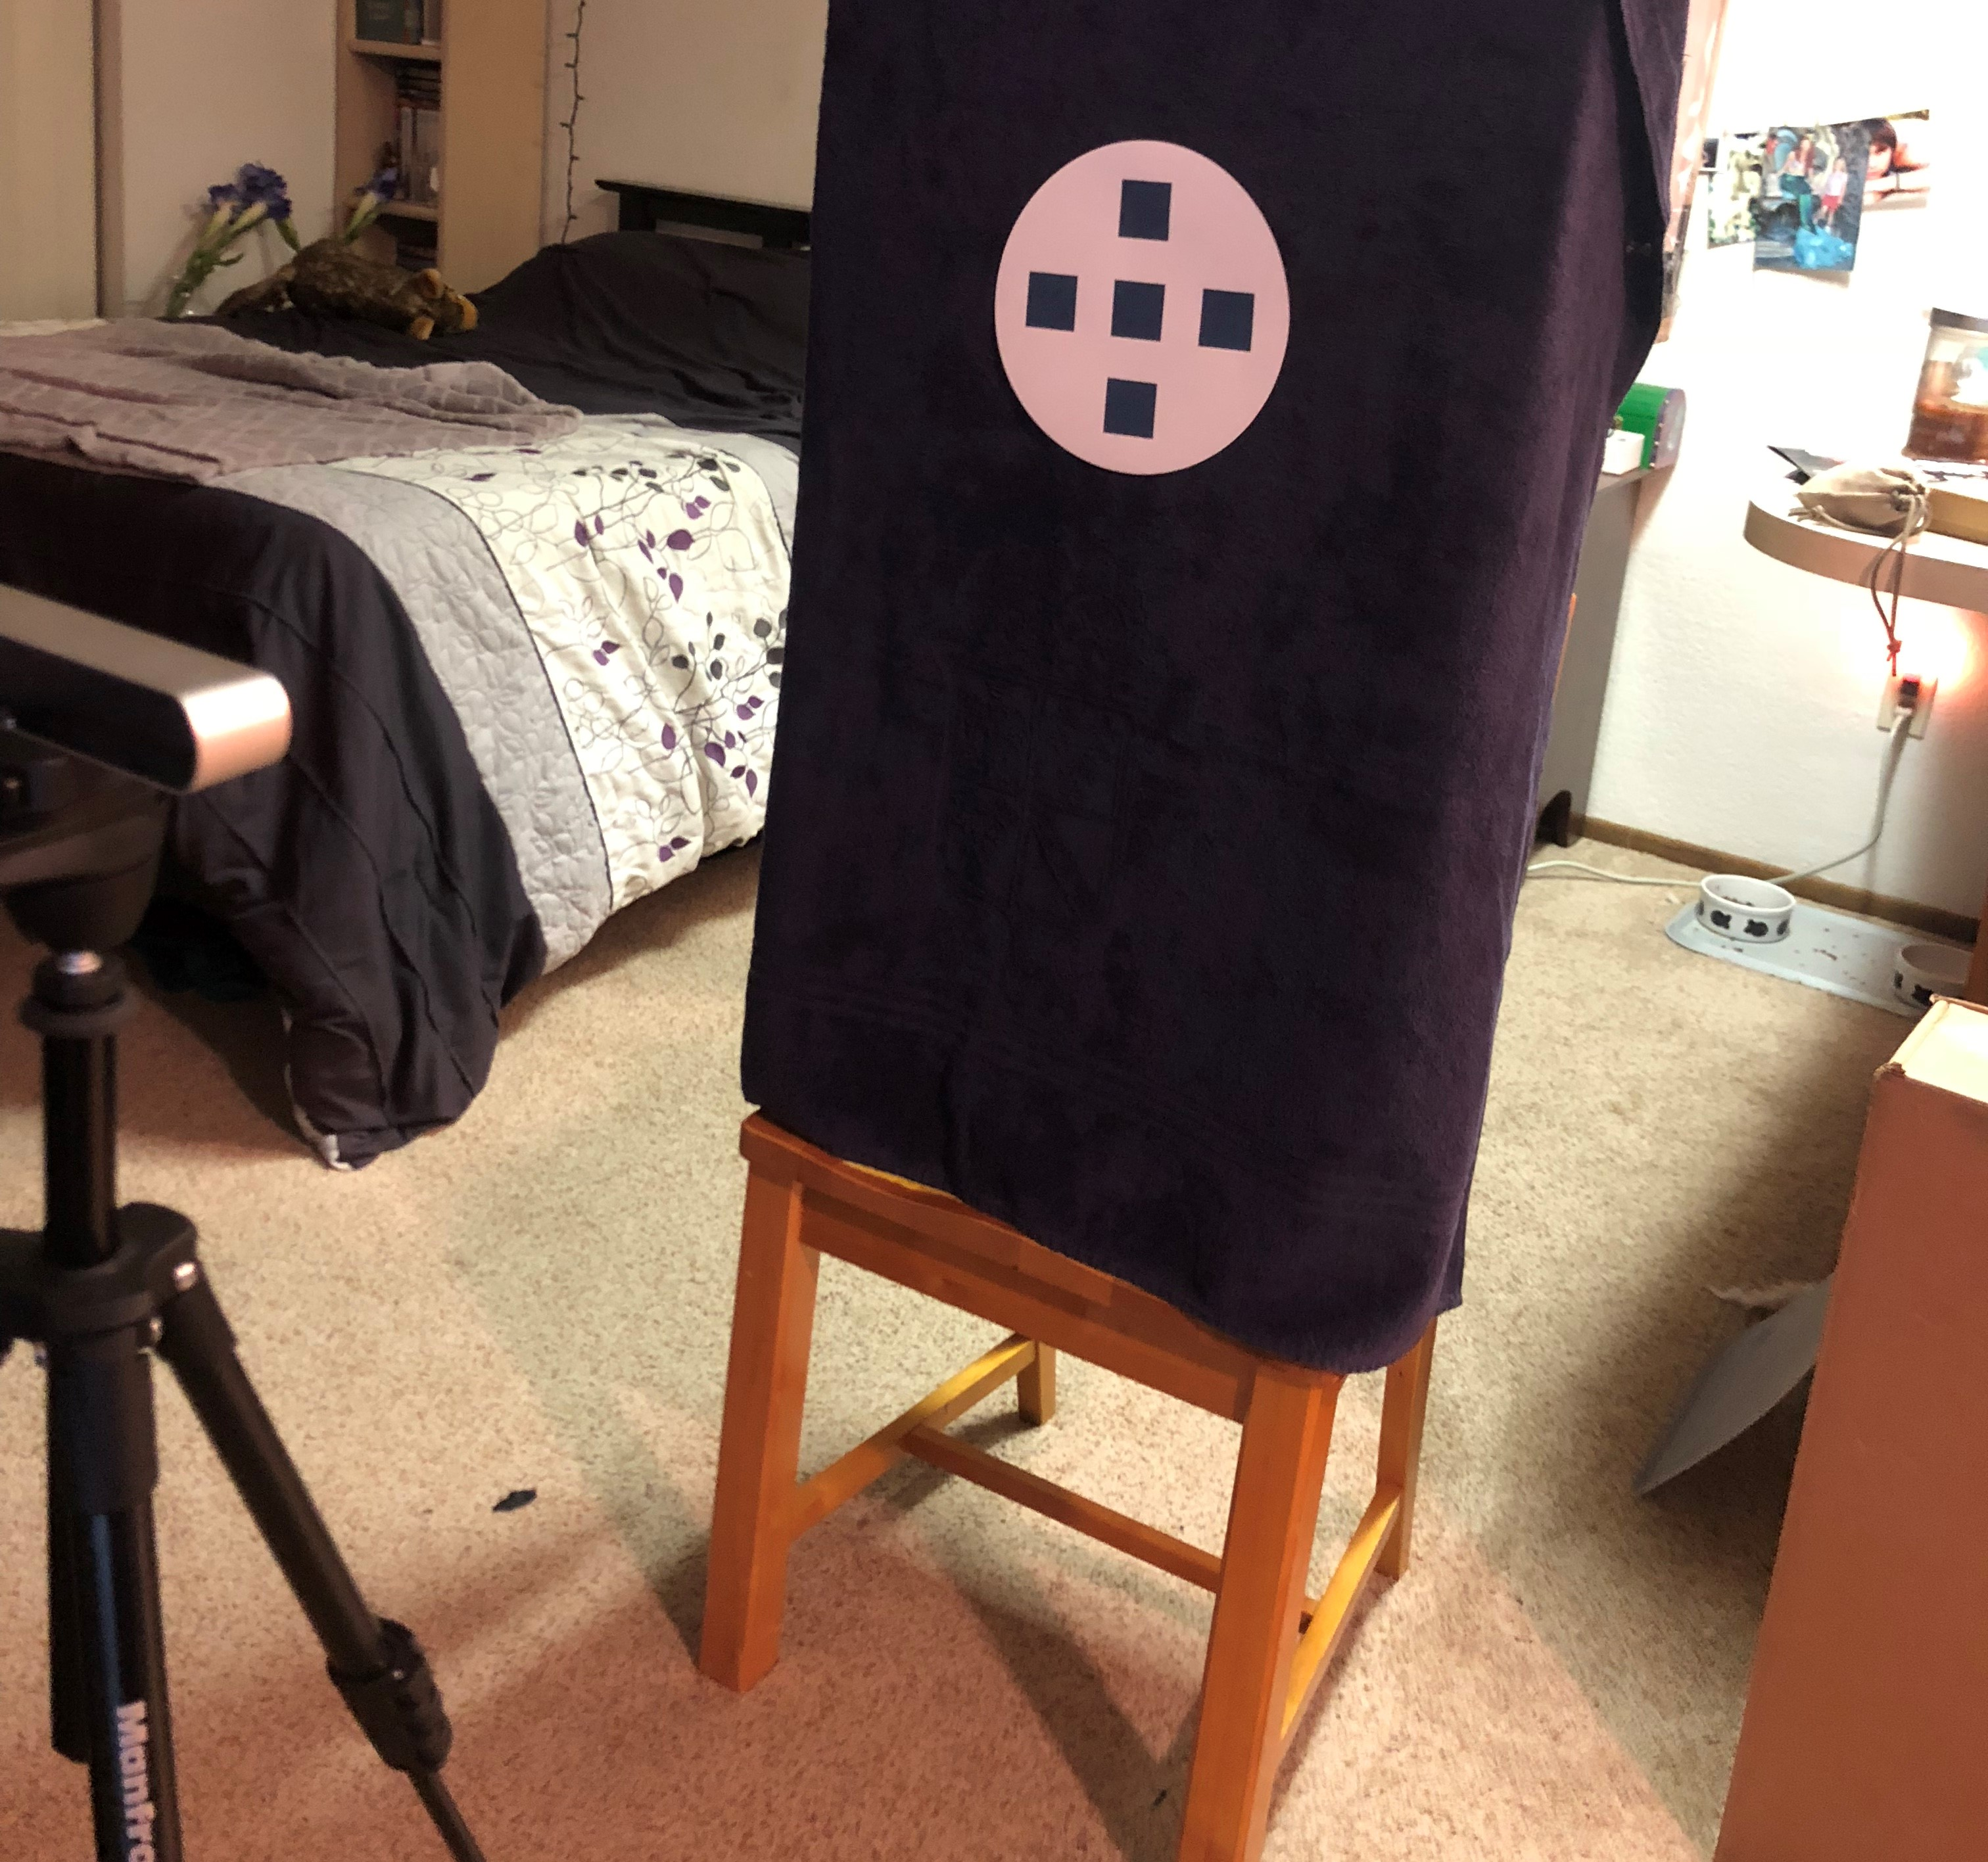
\includegraphics[width=5cm, height=5cm]{images/image1.jpeg}
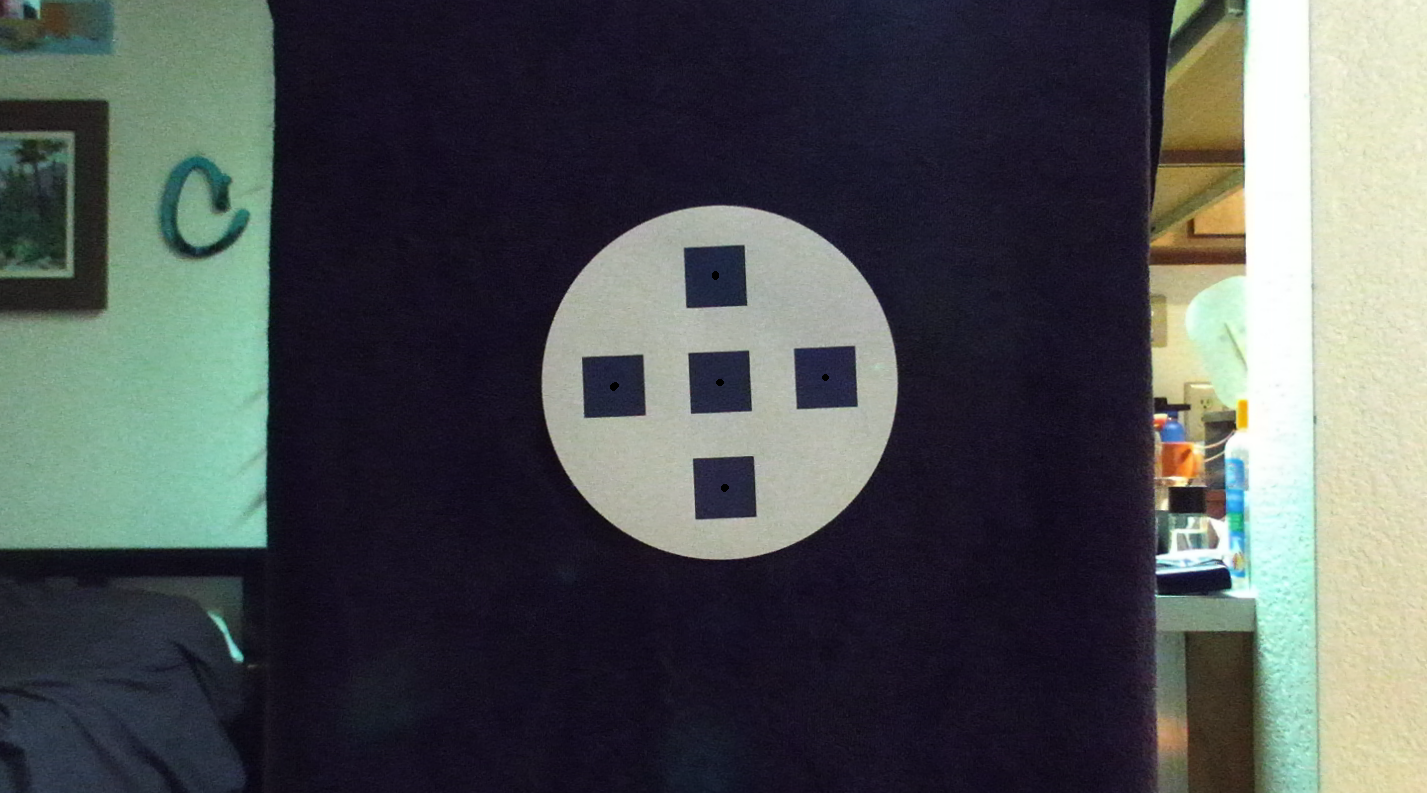
\includegraphics[width=9cm, height=5cm]{images/sample.PNG}

\subsection{Depth Measurements}
We are using a ZED camera to make our depth measurements.  This works down to a millimeter accuracy in good lighting on an NVIDIA GPU with compute capability of 3.0 or greater.  The software being used for this section is from the ZED SDK libraries. Our current build uses the ZED camera to pipe images to our opencv libraries which in turn collect distance data and send it back through the Zed libraries. This is then sorted for each point of the above diagram. Giving us a left, right, top, bottom, and center variable. From there that data can be used however is needed.

\subsection{Post Measurements}
The beta build includes libraries to accommodate our measurements once they are taken.  These calculations are responsible for calculating the track, axle width, Camber, and Tow.  


\section{To-Do's}
Our to do list consists of a few things at this point. We have beta functionality but would like to make improvements as we go onto spring term. First off, we plan to put together a better testing setup, as our current setup has very inconsistent lighting and other objects that our camera could potentially pick up. This makes it hard to maintain accuracy and repeat-ability. Our distance measurements at this point are very precise down to a couple millimeters. We know however, that our system has had some issues with poor setup and grabbing squares that were unintended. This was improved with better angling and bringing objects closer. There is room for improvement, but we are on the right track. We planned to make a custom fiducial but were held up by problems with setting up our stereo camera to work with the SDK. So seeing as that was a stretch goal, it was placed on the back burner. Finally we are going to receive a set of actual race car wheels we can use to recreate a more real world testing environment.

We have stretch goals as well. Our primary goal is to get error and rechecking hard-coded and out of the hand of any user. If we are able to identify if an error was made based on common issues we could inform the user and in some cases correct it for them. For example, we plan to detect that the markers captures are in the shape of a plus or an x. That way we could inform the user if we detected a square outside of our intended range and retry. We would also like to implement a portable development setup to fine tune our system when used outdoors and in different conditions. This would be done using an external GPU and a laptop that can connect via thunderbolt 3. We have an external GPU but still require a laptop that can connect via thunderbolt. This is not an essential goal but would make development much more convinient. 

\subsection{Error Checking}
We need to implement a more graceful error checking system into our project.  Occasionally our project can run into a few errors, in which case it halts the program or gives incorrect information.  For instance, if our program finds six squares instead of the intended five, it will typically count that sixth square as the top, left, right, or bottom square, and display the depth measurement for that instead.  We plan on implementing an error system which will restart the application when that error occurs, and potentially after a few tries, display to the user that the current environment is unstable for grabbing measurements.  Other errors that occur should print messages to the user and either prompt a restart or gracefully exit the program with a clear reason of faliure.


\subsection{Fiducials}
Our system uses clean squares as reference points. We plan to implement custom fiducials as a way to prevent false marker detection from opencv.  These custom fiducials would have a more unique design, which would keep our program from falsely choosing other contours and seeing them as needed measurements.

\subsection{User Interface}
Our user interface is purely how the data is printed once our program has completed running. This will be improved with a better error system down the road, and possibly a log file of past measurements and detected photos, that a user can go back through and read.

\section{Obstacles}
\noindent The majority of this term we were faced with the challenge of learning the new technology we transitioned to. This took up a considerable about of time as we were starting from fresh. Our solution throughout this term, though very predictable, has been researching proper use of openCV and understanding the math behind creating a depth map. However once we received a ZED stereo camera, we were able to use ZED's SDK and libraries to forgo the process of creating depth maps manually. This allowed us to focus on creating a wrapper that will use our openCV software with existing Nvidia libraries to measure the base information we need to input into our calculation functions. The only outstanding obstacle we face, other than further testing and research, is ensuring that the hardware we are using our software on includes an Nvidia graphics card with compute capability better than 3.0. At this point we have been doing testing on desktops in our homes, which has been a hamper on team based testing. The solution to this is to setup an external Nvidia GPU to use with a laptop or a portable workstation during development.

\section{Retrospective}
\begin{longtable}{ | p{0.075\linewidth} | p{0.3\linewidth} | p{0.3\linewidth} | p{0.3\linewidth} |} \hline
Weeks & Started & Continued & Actions  \\ \hline
1 & Setup meeting time with client for the following week. & Continued research about stereo vision started over winter break. & Setup regular meeting time for group and TA. \\ \hline
2 & Gathering a better understanding on our requirements from TA after our stereo vision adjustment. & Researching opencv to use with depth maps. Researching the manual acquisition of a depth map using two cameras. & Narrowed down previously established goals to essentials. \\ \hline
3 & Elevator pitch and poster draft. 
Developing code for fiducial acquisition using opencv in c++.
 & Research on depth map generation. Making alterations to our poster to prepare for next week’s poster review. & Practised our elevator pitch. 
Got a better understanding of presenting to different demographics. \\ \hline
4 & None. & Poster alterations, code research on depth maps, developing opencv and fiducial capturing. & Poster review was delayed due to inclement weather. Setup time for next week. \\ \hline
5 & Poster review gave us good feedback to take our layout and presentation. Started redesign draft. & Further code development for opencv and fiducial acquisition. Finding outline consistently. Need to work on finding center next. & Reached out to Kevin about stereo camera and answered some rudimentary questions. \\ \hline
6 & Started code base for ZED camera in a separate library. & Testing code to acquire fiducials on imputed images. Consistently finding centers on photos we tested.  & Acquired ZED stereo camera. Finished alpha level libraries for calculations and opencv libraries. ZED camera removed the need to manually create depth maps. \\ \hline
7 & At home testing of ZED camera with opencv & Testing SDK software wrapper for ZED. & TA instructed us to reach out to Kevin about acquiring a GPU dock for developing on our laptops. \\ \hline
8 & Combining Zed software with opencv & Testing SDK software wrapper for ZED. & Acquired dock for thunderbolt 3 but was unable to use with current set of laptops. \\ \hline
9 & None & Testing SDK software wrapper for Zed with opencv(with some success this time). & Put mobile dev of software on back-burner for another time. At home dev is going well enough. \\ \hline
10 & Planning for final progress report began & Code dev connecting Zed SDK with opencv  & \\ \hline
\end{longtable}

\end{document}